\begin{figure}
    \centering
    \vspace{-1em}
    \begin{subfigure}[t]{0.35\linewidth}
        \centering
        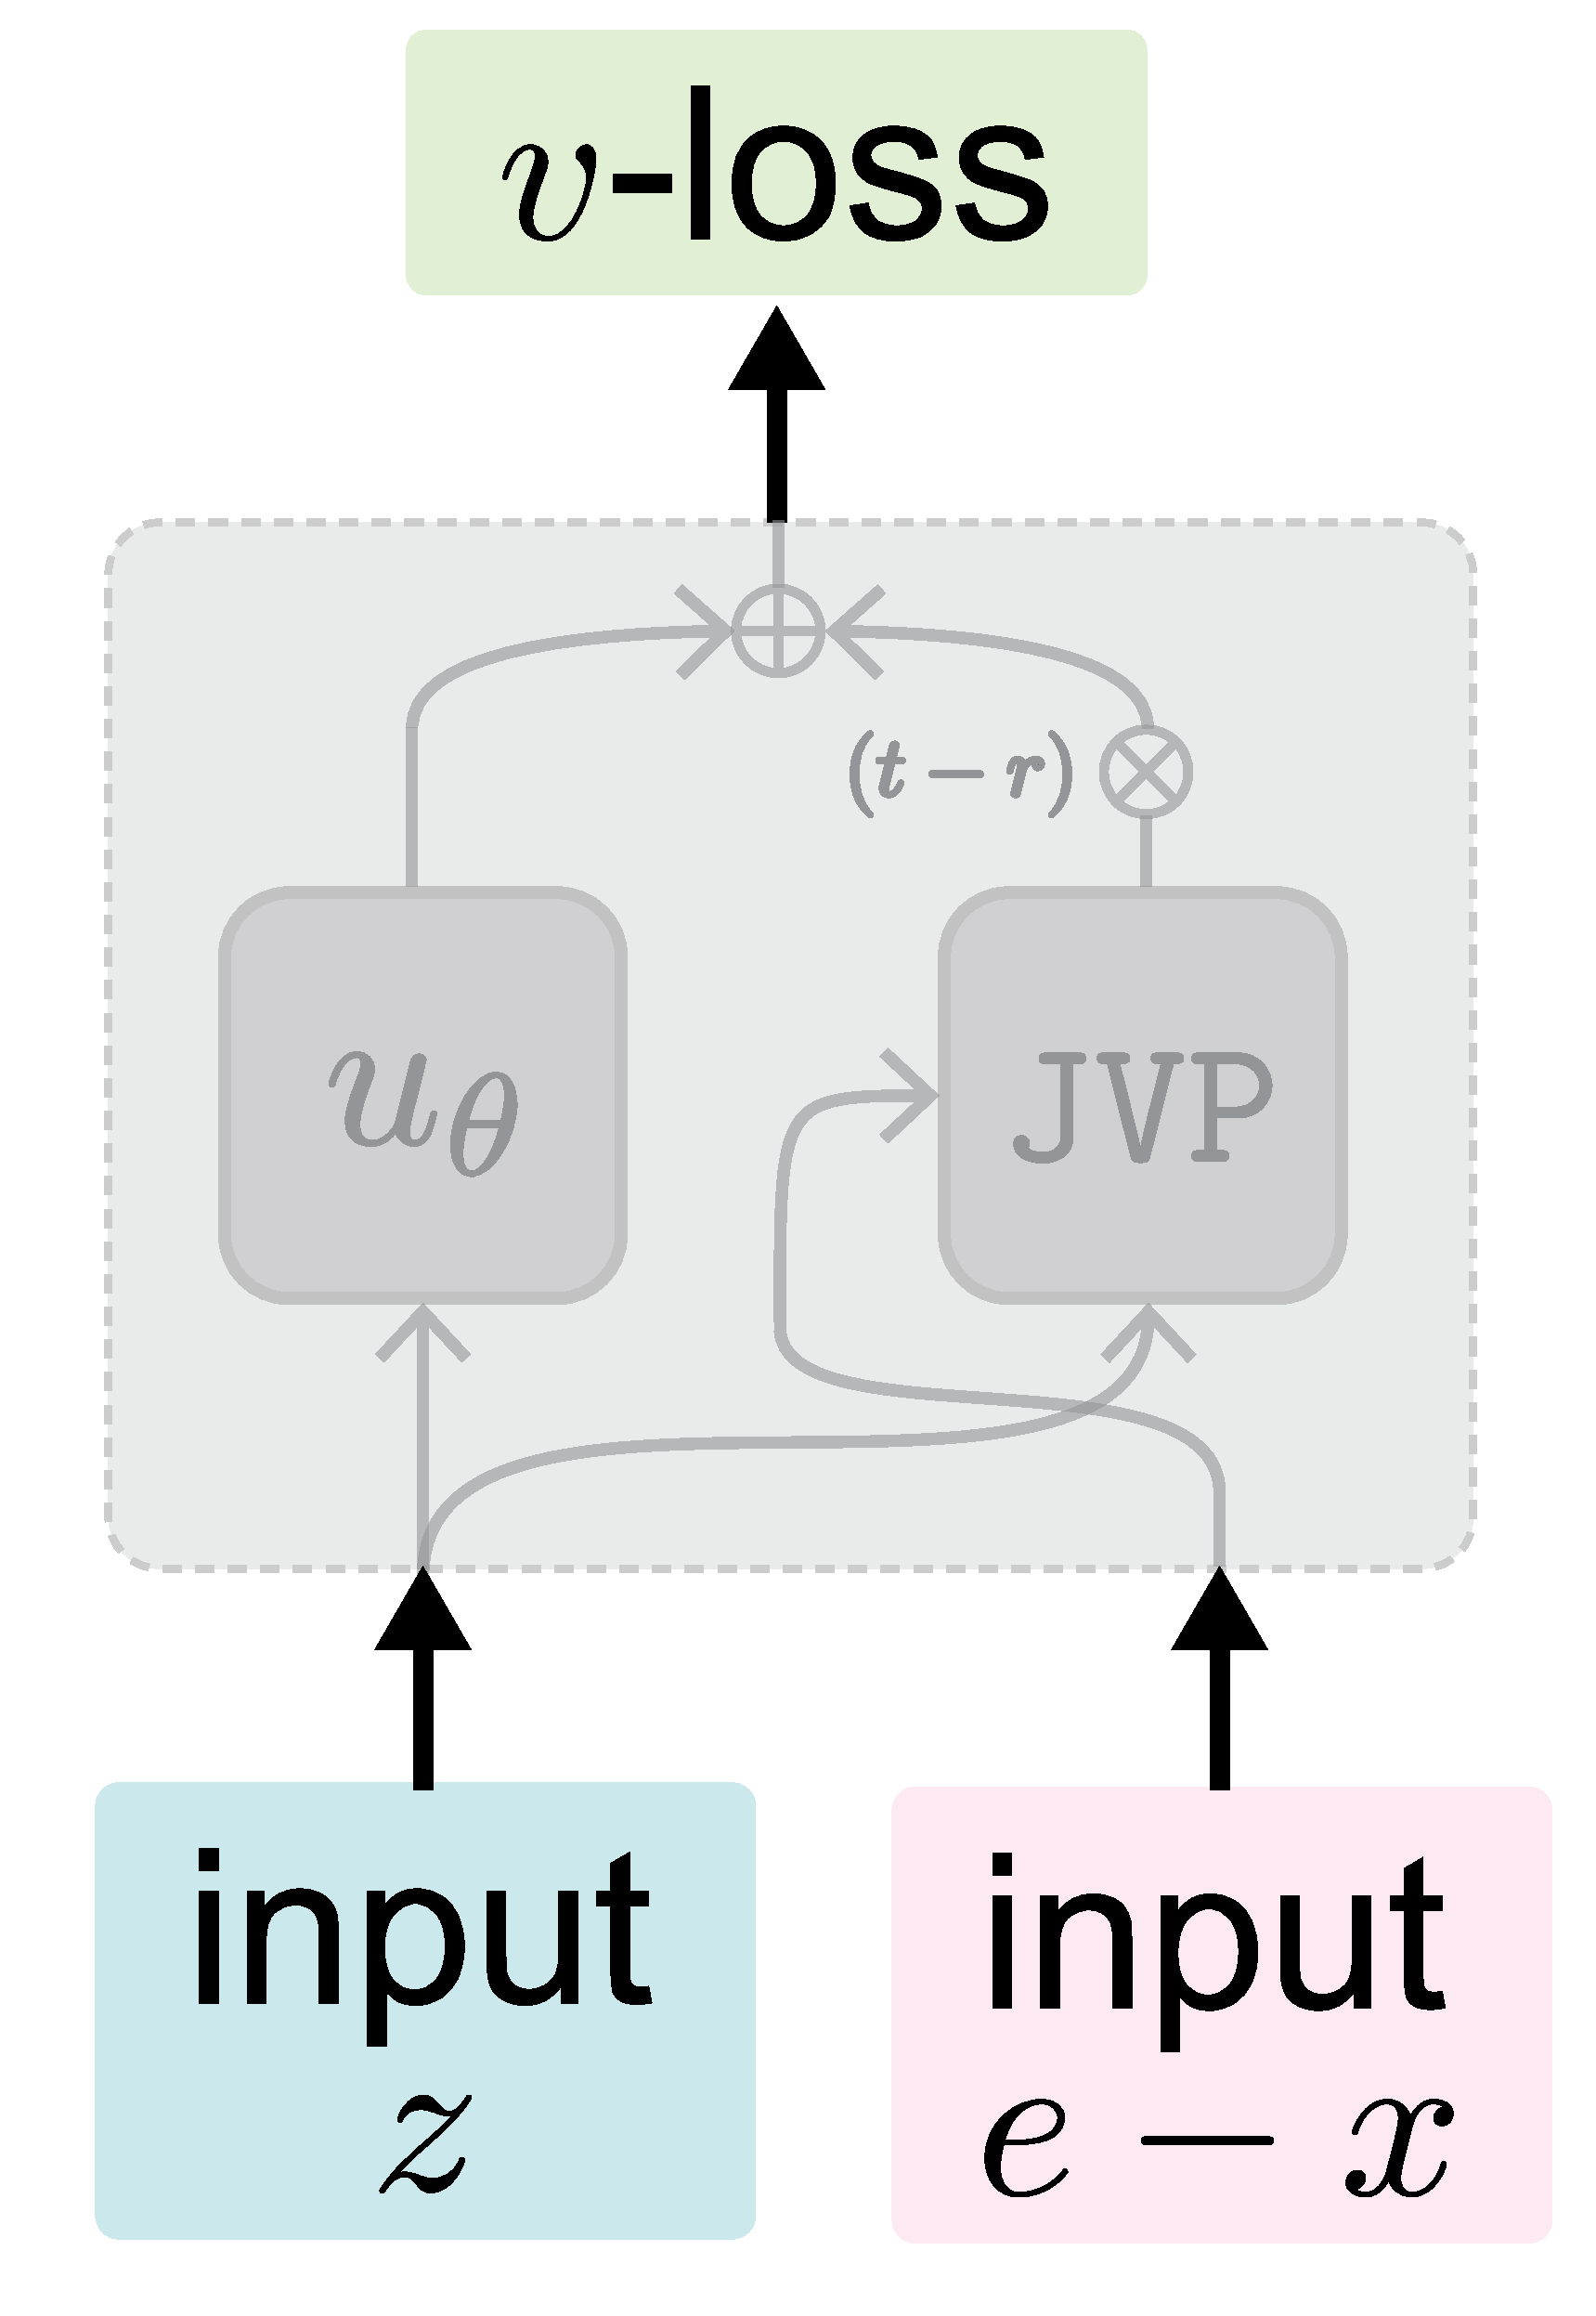
\includegraphics[width=\linewidth,clip,page=1]{figs/teaser.pdf}
        \caption{\centering Original MeanFlow}
        \label{fig:teaser_mf}
    \end{subfigure}
    \hspace{0.1\linewidth}
    \begin{subfigure}[t]{0.35\linewidth}
        \centering
        \includegraphics[width=\linewidth,clip,page=2]{figs/teaser.pdf}
        \caption{\centering Improved MeanFlow}
        \label{fig:teaser_imf}
    \end{subfigure}
    \vspace{-.2em}
    \caption{
    \textbf{Conceptual comparison}. Original MeanFlow (MF) \cite{mf} predicts \textit{average velocity} $u$ by a network $u_\theta$. As the ground-truth $u$ is unknown, original MF substitutes $u$ with the network's own prediction. We show that the original MF objective is equivalent to a loss on the \textit{instantaneous velocity} $v$ (namely, $v$-loss), but re-parameterized by the neural network $u_\theta$ (namely, $u$-pred), as shown in \textbf{(a)}. This re-parameterization, encompassed within the gray box, is determined by \textit{the MeanFlow identity} \cite{mf}.
    This reformulation reveals that the input to the compound function (in the gray box) is not only the noisy data (here, $z$), but also the conditional velocity ($e - x$), which is not a standard regression problem. In \textbf{(b)}, our improved objective is conceptually \emph{\textbf{$v$-loss re-parameterized by $u$-pred}}, taking only the legitimate input $z$.
    }
    \vspace{-.7em}
    \label{fig:teaser}
\end{figure}